\documentclass[11pt,a4paper]{ctexart}
\usepackage[margin=2.5cm]{geometry}
\usepackage{amsmath,amssymb,amsthm}
\usepackage{graphicx}
\usepackage{booktabs}
\usepackage{hyperref}
\usepackage{tikz}
\usepackage{xcolor}
\usepackage{listings}
\usetikzlibrary{positioning, fit, arrows.meta, calc, backgrounds, shapes.geometric}

\hypersetup{
  colorlinks=true,
  linkcolor=blue!60!black,
  citecolor=blue!60!black,
  urlcolor=blue!60!black,
}

\title{CrowdVarNet + PedPred 教师方案：模型框架详解}
\author{}
\date{}

\begin{document}
\maketitle

\section{概述}

本文档详细介绍当前最佳模型方案的整体框架。系统由两个解耦的子模型构成：

\begin{itemize}
  \item \textbf{教师模型 PedPred}（\texttt{pedpred3\_gru\_mid}）：基于稠密真值的预训练物理先验，预测下一帧人群状态分布；
  \item \textbf{学生模型 CrowdVarNet}：可微变分反演求解器，融合稀疏移动传感器观测与教师先验，恢复稠密的人群状态。
\end{itemize}

教师在 Phase 1 用 NLLL 损失独立预训，之后\textbf{完全冻结}；学生在 Phase 2/3 用 TBPTT（Truncated Backpropagation Through Time，截断时序反向传播）训练，期间教师作为外部 prior 不参与梯度更新。

\section{问题定义}

\subsection{物理场}

研究对象：日本大阪 ATC 商场走廊的人群流动。
状态被栅格化为 $H\times W = 60\times 96$ 网格（空间分辨率 $1\,\mathrm{m}$，时间分辨率 $1\,\mathrm{s}$）。
每格在每帧的状态由 $4$ 个通道描述：
\begin{equation}
\mathbf{x}_t \in \mathbb{R}^{4\times H\times W}, \quad
\mathbf{x}_t = \bigl(\log\rho,\,v_x,\,v_y,\,\log\sigma^2\bigr)
\end{equation}
其中 $\rho$ 为人群密度，$(v_x, v_y)$ 为速度均值场，$\sigma^2$ 为速度方差场。

\subsection{观测模型}

走廊内有 $N_a=3$ 个移动传感器（agent），各自半径 $r=5$ 格视野，每帧位置自动前进一格趋向预设目标。每帧的观测算子记为 $C_t$（稀疏 0/1 选择矩阵）：
\begin{equation}
\mathbf{y}_t = C_t \mathbf{x}_t + \boldsymbol{\eta}_t, \quad \boldsymbol{\eta}_t \sim \mathcal{N}(0,\Sigma_y)
\end{equation}
观测覆盖率约 $10\text{--}15\%$，背景大片像素完全不可见。

\subsection{反演任务}

对每个时刻 $t$，给定历史观测序列 $\{\mathbf{y}_\tau\}_{\tau\le t}$ 和历史状态估计 $\{\hat{\mathbf{x}}_\tau\}_{\tau< t}$，求当前最优稠密估计 $\hat{\mathbf{x}}_t$。

\section{教师模型 PedPred (\texttt{gru\_mid})}

\subsection{动机与定位}

教师只解决一个简单问题：\textbf{在已知稠密历史 $\mathbf{x}_{t-5..t-1}$ 的前提下，预测 $\mathbf{x}_t$}。
它不接触观测算子 $C_t$，因此可以脱离观测稀疏性单独训练。
学生再通过变分反演把它的输出和观测残差融合。

\subsection{结构}

PedPred 是 Encoder–Forecaster 架构。输入 $[B,5,4,H,W]$，输出 $[B,1,4,H,W]$。

\paragraph{Encoder}
三层下采样栈，每层 \textit{Conv2d} 后接 \textit{ConvGRU}：
\begin{equation*}
\begin{aligned}
&\text{Conv2d}_{4\to 24} \to \text{ConvGRU}(24)\\
&\to \text{Conv2d}_{\downarrow,\, 24\to 48} \to \text{ConvGRU}(48)\\
&\to \text{Conv2d}_{\downarrow,\, 48\to 192} \to \text{ConvGRU}(192)
\end{aligned}
\end{equation*}
ConvGRU 维度 $\{24, 48, 192\}$（v11 mid 配置）。
ConvGRU 提供时序记忆，下采样让感受野覆盖整个走廊。

\paragraph{Temporal-attn}
跨 5 帧聚合 hidden state，加权求和（attention over time）。

\paragraph{Forecaster}
对应的上采样栈：
\begin{equation*}
\text{ConvGRU}\to \text{ConvT2d}_\uparrow \to \text{ConvGRU} \to \text{ConvT2d}_\uparrow \to \text{ConvGRU} \to \text{Conv2d} \to \text{Conv2d}_{\to 4}
\end{equation*}
末层 $1\times 1$ Conv 把 feature 映射回 4 通道，并做 clamp（防数值溢出）：
\begin{equation*}
\log\rho \in [-20, 10], \quad
v_x, v_y \in [-15, 15], \quad
\log\sigma^2 \in [-20, 5]
\end{equation*}

\paragraph{参数量} 约 $7 \times 10^6$（不参与学生训练时的梯度）。

\subsection{NLLL 损失}

教师的关键设计选择是用\textbf{高斯负对数似然损失（NLLL）}训练，而非简单 MSE。设预测为 $(\hat\mu, \hat\sigma^2)$，则速度通道损失：
\begin{equation}
\mathcal{L}_v = \frac{1}{2|\Omega|}\sum_{i\in\Omega}
\Bigl[
\frac{(v_{i,\mathrm{gt}} - \hat\mu_i)^2}{\hat\sigma_i^2}
+ \log \hat\sigma_i^2
\Bigr]
\end{equation}
$\Omega$ 是软掩码（密度 $>$ threshold 的像素）。

NLLL 让模型自适应分配方差：噪声大的像素自动被赋大 $\hat\sigma^2$，相当于自适应样本权重。
对比 MSE 训练版本，NLLL 在 valid 集 vx/vy support-RMSE 改善 $25\text{--}30\%$。

\subsection{训练超参}

\begin{itemize}
  \item Optimizer: AdamW, lr $=5\times 10^{-4}$, weight\_decay $=10^{-4}$
  \item Batch size 48, 30 epoch
  \item 数据增广：W 轴翻转（同时 $v_x \to -v_x$），概率 0.5
  \item Early stopping patience 20
  \item 输入 \texttt{nin}=5 帧, 输出 \texttt{nout}=5 帧
\end{itemize}

\subsection{性能}

教师在 valid 集（support pixels, $\rho > 0.05$）的 RMSE：
\begin{center}
\begin{tabular}{lc}
\toprule
通道 & support\_RMSE \\
\midrule
$\rho$    & 0.129 \\
$v_x$     & 0.277 \\
$v_y$     & 0.232 \\
\bottomrule
\end{tabular}
\end{center}

$v_y$ 已逼近数据噪声地板（估计 $\sim 0.20$），物理上无更多优化空间。

\section{学生模型 CrowdVarNet}

\subsection{变分反演框架}

学生在每个时间步隐式求解
\begin{equation}\label{eq:varprob}
\hat{\mathbf{x}}_t = \arg\min_{\mathbf{x}}\;
\underbrace{\lVert C_t\mathbf{x} - \mathbf{y}_t \rVert_{R}^2}_{\text{观测项}}
+\underbrace{w_{\text{prior}}\,\lVert\mathbf{x} - \boldsymbol{\phi}_t\rVert^2}_{\text{先验项}}
\end{equation}
其中 $\boldsymbol{\phi}_t = \mathrm{PedPred}(\hat{\mathbf{x}}_{t-5..t-1})$ 是教师对当前帧的预测，$w_{\text{prior}}=0.5$（已扫优）。

\subsection{学习的 Proximal Operator}

直接闭式解不可得（$C_t$ 稀疏 + $\boldsymbol{\phi}$ 是非凸网络）。
我们用一个 \textbf{ConvGRU 求解器}做 $n_{\text{iter}}=8$ 次迭代展开：
\begin{equation}
\delta\mathbf{x}^{(k)} = \mathrm{ConvGRU}_\theta\Bigl(
\mathbf{x}^{(k-1)},\,
C_t^{\!\top}(\mathbf{y}_t - C_t\mathbf{x}^{(k-1)}),\,
w_{\text{prior}}(\mathbf{x}^{(k-1)}-\boldsymbol{\phi}_t)
\Bigr)
\end{equation}
\begin{equation}
\mathbf{x}^{(k)} = \mathbf{x}^{(k-1)} + \delta\mathbf{x}^{(k)}, \quad
\hat{\mathbf{x}}_t = \mathbf{x}^{(8)}
\end{equation}
ConvGRU 隐藏维度 256，卷积核 $3\times 3$，dropout 0.1。
求解器学习的是 \textit{learned proximal operator}：把展开优化的更新规则参数化进网络。

\paragraph{参数量} 求解器约 $2 \times 10^6$（教师冻结，不计入）。

\subsection{初始猜测}

\begin{itemize}
  \item 第一个时间步：$\mathbf{x}^{(0)}_t = \boldsymbol{\phi}_t$（直接用教师预测做起点）
  \item 后续时间步：$\mathbf{x}^{(0)}_t = \hat{\mathbf{x}}_{t-1}$ + 教师增量
  \item 可选 \texttt{init\_gate}：可学习融合门把 $\boldsymbol{\phi}_t$ 和 $\hat{\mathbf{x}}_{t-1}$ 加权混合
\end{itemize}

\section{框架图}

\begin{figure}[h]
\centering
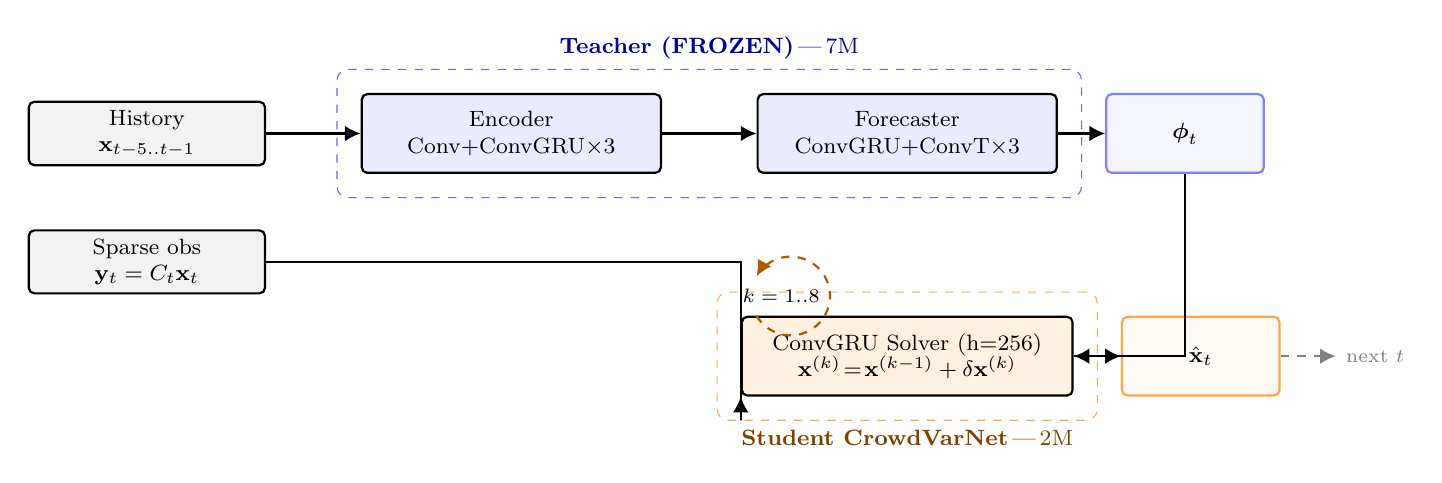
\begin{tikzpicture}[
  font=\footnotesize,
  node distance=8mm and 12mm,
  >={Latex[length=2mm,width=2mm]},
  block/.style={
    draw=black, thick, rounded corners=2pt,
    align=center, minimum height=10mm, inner sep=3pt
  },
  teacher/.style={block, fill=blue!8,  minimum width=38mm},
  solver/.style ={block, fill=orange!12, minimum width=42mm},
  io/.style     ={block, fill=gray!10, minimum width=30mm, minimum height=8mm},
  loop/.style   ={draw=orange!70!black, thick, dashed, rounded corners=4pt},
]

\node[io] (hist) {History\\$\mathbf{x}_{t-5..t-1}$};
\node[io, below=of hist] (obs)
  {Sparse obs\\$\mathbf{y}_t = C_t \mathbf{x}_t$};

\node[teacher, right=of hist] (enc)
  {Encoder\\Conv+ConvGRU$\times 3$};
\node[teacher, right=of enc] (fore)
  {Forecaster\\ConvGRU+ConvT$\times 3$};
\node[block, fill=blue!4, draw=blue!50,
      right=6mm of fore, minimum width=20mm]
      (prior) {$\boldsymbol{\phi}_t$};

\begin{scope}[on background layer]
\node[fit=(enc)(fore), draw=blue!60, dashed,
      rounded corners=4pt, inner sep=3mm,
      label={[blue!60!black]above:\textbf{Teacher (FROZEN)}\,---\,7M}]
      (teacher_box) {};
\end{scope}

\node[solver, below=18mm of fore] (solver)
  {ConvGRU Solver (h=256)\\
   $\mathbf{x}^{(k)} \!=\! \mathbf{x}^{(k-1)}+ \delta\mathbf{x}^{(k)}$};
\node[block, fill=orange!4, draw=orange!70,
      right=6mm of solver, minimum width=20mm]
      (out) {$\hat{\mathbf{x}}_t$};

\begin{scope}[on background layer]
\node[fit=(solver), draw=orange!70, dashed,
      rounded corners=4pt, inner sep=3mm,
      label={[orange!50!black]below:\textbf{Student CrowdVarNet}\,---\,2M}]
      (student_box) {};
\end{scope}

\draw[->, thick] (hist) -- (enc);
\draw[->, thick] (enc)  -- (fore);
\draw[->, thick] (fore) -- (prior);
\draw[->, thick] (prior.south) |- (solver.east);
\draw[->, thick] (obs.east) -| ($(solver.south west)+(0,-3mm)$) -- (solver.south west);
\draw[->, thick] (solver) -- (out);
\draw[loop, ->] (solver.north west) ++(2mm,0) arc (-150:150:5mm)
  node[midway, left, font=\scriptsize] {$k=1..8$};
\draw[->, gray, thick, dashed]
  (out.east) -- ++(7mm,0) node[right] {\scriptsize next $t$};

\end{tikzpicture}
\caption{整体框架图。蓝色虚框为冻结教师，橙色虚框为学生求解器。}
\label{fig:arch}
\end{figure}

\section{学生训练：TBPTT}

\subsection{挑战}

学生在多个时间步串联：$\hat{\mathbf{x}}_t$ 依赖之前所有 $\hat{\mathbf{x}}_{<t}$（通过 history $\to$ teacher $\to$ prior 链），ConvGRU 求解器又有自己的 hidden state。
完整 BPTT 在 episode 长度 $T=600$ 时显存爆炸（每帧 8 次迭代，反向链 $\sim 4800$）。

\subsection{TBPTT 解法}

每 $k'=12$ 帧反向一次、清梯度，但 hidden state 继续往前（detach 不传梯度）：
\begin{equation*}
\underbrace{\text{frame } 1\text{--}12}_{\text{backward, step}}
\;\to\;
\underbrace{\text{frame } 13\text{--}24}_{\text{backward, step}}
\;\to\;
\cdots
\;\to\;
\underbrace{\text{frame } T-11\text{--}T}_{\text{last window}}
\end{equation*}
$T/k' = 50$ 次反向 / episode；模型仍学到 $T$ 步长程依赖（hidden state 跨窗连续），只是反向被截断。

\subsection{两阶段训练}

\paragraph{Stage 2-a: 单步主训}（25 epoch 预算）
\begin{itemize}
  \item episode\_len = 300, $k'=8$
  \item batch 48, lr $=2\times 10^{-4}$, cosine 衰减
  \item channel weights $(\rho, v_x, v_y, \sigma^2) = (3.0, 1.5, 1.0, 0)$（$\sigma^2$ 不监督）
  \item warmup 5 帧（用 GT），之后用学生输出 feedback
  \item EMA $\beta=0.999$, dropout 0.1, grad-clip 0.5
  \item flip-W 增广，概率 0.5
\end{itemize}
最佳 val\_rollout\_loss = 0.0550（epoch 10 后 plateau）。

\paragraph{Stage 3: 长 horizon 微调}（关键收益）
\begin{itemize}
  \item warmstart 自 Stage 2-a 的 best.pt
  \item episode\_len = 600（双倍）, $k'=12$（1.5×）
  \item lr 降至 $5\times 10^{-5}$, 8 epoch
\end{itemize}
6 epoch 即把 val 压到 \textbf{0.04738}（相对单步 baseline 改善 \textbf{13.9\%}）。

学生的瓶颈不在单步精度，而在多步外推鲁棒性 —— 长 episode 训练让 ConvGRU 求解器学到更稳定的 hidden state 演化。

\section{推理流程}

\begin{enumerate}
  \item 用 5 帧 GT warm-up（部署时用前 5 帧观测最近邻补齐）；
  \item 对每个 $t \ge 5$：
    \begin{enumerate}
      \item 当前 agent 位置生成 $C_t$，得稀疏观测 $\mathbf{y}_t$；
      \item 教师 forward：$\boldsymbol{\phi}_t = \mathrm{PedPred}(\hat{\mathbf{x}}_{t-5..t-1})$；
      \item 求解器 8 次迭代：$\hat{\mathbf{x}}_t = \mathbf{x}^{(8)}$；
      \item 输出 $\hat{\mathbf{x}}_t$ 并加入 history 缓冲；
    \end{enumerate}
\end{enumerate}

\paragraph{速度} 单帧 $\sim 0.56$\,s（V100），即 1.8\,Hz；H100/H200 上估计 $\sim 0.3$\,s。
对 1\,Hz 实时人群监控有充裕余量。

\section{关键超参一览}

\begin{center}
\begin{tabular}{lll}
\toprule
组件 & 参数 & 取值 \\
\midrule
\multirow{4}{*}{Teacher} & objective & nlll \\
                         & arch     & pedpred3\_gru\_mid \\
                         & hidden GRU & (24, 48, 192) \\
                         & params   & 7\,M \\
\midrule
\multirow{4}{*}{Student solver} & solver-type & convgru \\
                                & solver-hidden & 256 \\
                                & solver-kernel & 3 \\
                                & n\_iter (展开) & 8 \\
\midrule
\multirow{2}{*}{Variational}  & w\_prior   & 0.5 \\
                              & rho-mask-thr & 0.05 \\
\midrule
\multirow{4}{*}{Training (S3)} & episode\_len & 600 \\
                               & $k'$ (TBPTT) & 12 \\
                               & lr           & $5\times 10^{-5}$ \\
                               & ch\_weights  & (3, 1.5, 1, 0) \\
\midrule
\multirow{2}{*}{Sensors} & num\_agents     & 3 \\
                         & sensing-range   & 5 grid cells \\
\bottomrule
\end{tabular}
\end{center}

\section{Checkpoint 路径}

\begin{itemize}
  \item Teacher: \texttt{runs/pedpred\_v13\_gru\_mid\_nlll\_17843926/checkpoints/free-pig\_best.hkl}
  \item Student: \texttt{runs/cvn\_p3\_v13\_horizon\_17847842/best.pt}
\end{itemize}

\section{相关已封顶的尝试}

下列方向均经实验验证\textit{未带来明显收益}：
\begin{itemize}
  \item 教师 cos 方向损失：$<1\%$；
  \item 速度残差预测 + vx 损失加权：$<1\%$；
  \item Wide CNN backbone：教师略优但学生方差更大；
  \item $w_{\text{prior}}=1.0$：val 变差 $5\%$；
  \item 解冻教师末两层联合微调：val 变差 $12\%$（扰乱 $\log\sigma^2$ 学习）；
  \item 学生单步训练 plateau 后续训：$<1.5\%$；
\end{itemize}

总结：当前架构已接近本数据集物理与算法的双重边界。
$v_y$ 距噪声地板仅 $\sim 15\%$，$v_x$ 仍有 $5\text{--}10\%$ 空间。

\end{document}
